
\pagebreak
\section{GUIs}
Matlab has a handy tool for developing GUIs (guide) that will meet most of your needs.
 You can also bulid a gui programatically, which affords you more control over element placement.

\subsection{Guide}
Launch guide by typing ''guide'' into the command line.
 You can then build your GUI using their GUI interface.
 After you save your GUI figure, Matlab will generate a .m file with a code outline.
 You can them modify this code outline to perform your tasks.
 Objects in your GUI are referred to in the code by their 'tag'.
 The handles to all of these objects are stored in a 'handles' variable.
 So in the code below you'll find frequent references to code that looks like; ''handles.tag''.
 These access the elements in the GUI.

When you need to run the GUI, run the .m file, not the figure.

\begin{figure}[ht!]
\centering
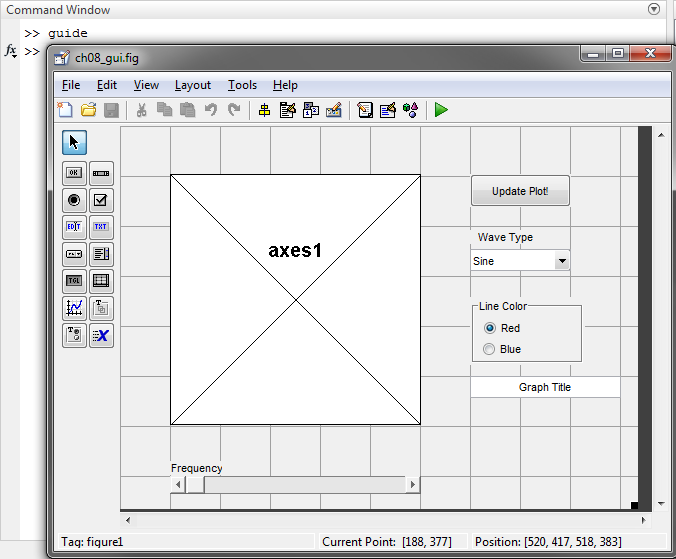
\includegraphics[width=120mm]{img/guide.png}
\caption{Guide and it's invocation.
 The menu on the left allows you to add components.
 Double click a component to view it's properties}
\label{guiload}
\end{figure}

\pagebreak
Here is the code for the GUI.
 I have removed many of the auto-generated comments.
 What are contained here are the 'callbacks' the functions that are called when the user interacts with the GUI elements.
 The code that actually performs most of the plotting is separated into the function ''ch08updatePlot.m'.
 This practice reduces duplicate code, and allows for easier debugging of complex GUIs.
 You can find the update function in the next section.

\begin{quote}
\verbatiminput{code/ch08_gui.m}
\end{quote}

\pagebreak
This function updates the GUI in the previous section.
 I've separated it here so you can see the core functions of the GUI seaparated from the callbacks.

\begin{quote}
\verbatiminput{code/ch08_updatePlot.m}
\end{quote}

\pagebreak
\subsection{Manually}
It is also possible to generate a GUI programatically.

\begin{quote}
 \verbatiminput{code/ch08_guimanual.m}
\end{quote}
